% ថ្នាក់ទី ១១ (វិទ្យាសាស្ត្រសង្គម) · ជំពូកទី ៣ · មេរៀនទី ៤ · សៀវភៅ ទំព័រ ១០៨–១២៤
\chapter{សមីការនិងវិសមីការត្រីកោណមាត្រ}

\begin{objBox}[វត្ថុបំណង]
\begin{enumerate}[1]
  \item ដោះស្រាយសមីការត្រីកោណមាត្រ
  \item ដោះស្រាយវិសមីការត្រីកោណមាត្រ ។
\end{enumerate}
\end{objBox}

\section{ចំនួនដែលមានកូស៊ីនុសដូចគ្នា}

គេឱ្យពីរចំនួន $x$ និង $y$ ដែលមានកូស៊ីនុស $\cos x = \cos y$ ដូចគ្នា ។ ក្នុងរង្វង់ត្រីកោណមាត្រដែលមានផ្ចិត $O$ គេមាន $M$ និង $N$ ជាចំណុចនៅលើរង្វង់ដែលមុំ $(\overrightarrow{OA}, \overrightarrow{ON}) = y$ និងមុំ $(\overrightarrow{OA}, \overrightarrow{OM}) = x$ ។
\begin{center}
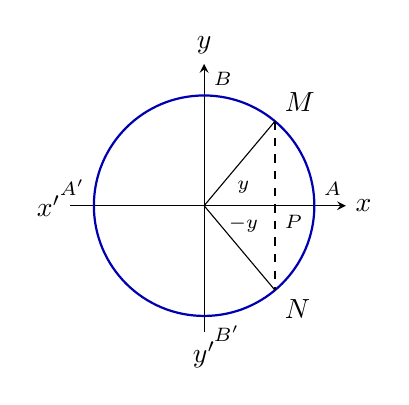
\begin{tikzpicture}[scale=1,>=stealth]
  \draw[->] (-1.7,0) -- (1.8,0) node[right] {$x$};
  \draw[->] (0,-1.6) -- (0,1.8) node[above] {$y$};
  \node[left] at (-1.7,0) {$x'$}; \node[below] at (0,-1.6) {$y'$};
  \draw[blue!70!black,thick] (0,0) circle (1.4);
  \draw (0,0) -- (50:1.4) node[above right] {$M$};
  \draw (0,0) -- (-50:1.4) node[below right] {$N$};
  \draw[dashed] (50:1.4) -- (-50:1.4);
  \node[below right] at (0.9,0) {\scriptsize $P$};
  \node[above right] at (1.4,0) {\scriptsize $A$}; \node[above left] at (-1.4,0) {\scriptsize $A'$};
  \node[above right] at (0,1.4) {\scriptsize $B$}; \node[below right] at (0,-1.4) {\scriptsize $B'$};
  \node at (25:0.55) {\scriptsize $y$}; \node at (-25:0.55) {\scriptsize $-y$};
\end{tikzpicture}
\end{center}
អាប់ស៊ីសនៃចំណុច $N$ គឺ $\cos y$ ។ ដោយ $\cos x = \cos y$ នោះ ចំណុច $M$ និង $N$ មានអាប់ស៊ីសដូចគ្នា ។ ដូច្នេះ គេបានករណីពីរដូចខាងក្រោម ៖
\begin{itemize}
  \item បើ $M$ និង $N$ ត្រួតស៊ី នោះ $x$ និង $y$ ជារង្វាស់មុំតែមួយ ។ ដូច្នេះ $x = y + 2k\pi$ \ $(k \in \mathbb{Z})$ ។
  \item បើ $M$ និង $N$ ឆ្លុះគ្នាធៀបនឹងអ័ក្ស $(x'x)$ នោះមុំ $(\overrightarrow{OA}, \overrightarrow{ON})$ និងមុំ $(\overrightarrow{OA}, \overrightarrow{OM})$ ជាមុំផ្ទុយគ្នា ហើយ $-y$ ជារង្វាស់មួយនៃមុំ $(\overrightarrow{OA}, \overrightarrow{OM})$ ។ ដូច្នេះ $x = -y + 2k\pi$, $(k \in \mathbb{Z})$ ។
\end{itemize}
\begin{formulaBox}[ជាទូទៅ]
គេបាន (I) ពីរចំនួន $x$ និង $y$ មានកូស៊ីនុសដូចគ្នា $\cos x = \cos y$ លុះត្រាតែ $x = y + 2k\pi$ ឬ $x = -y + 2k\pi$, $(k \in \mathbb{Z})$ ។
\end{formulaBox}

\section{ចំនួនដែលមានស៊ីនុសដូចគ្នា}

គេឱ្យពីរចំនួន $x$ និង $y$ មានស៊ីនុសដូចគ្នា $\sin x = \sin y$ ។ ក្នុងរង្វង់ត្រីកោណមាត្រមានផ្ចិត $O$ ចំណុច $M$ និង $N$ ជានៅលើរង្វង់ដែលមុំ $(\overrightarrow{OA}, \overrightarrow{ON}) = y$ និងមុំ $(\overrightarrow{OA}, \overrightarrow{OM}) = x$ ។
\begin{center}
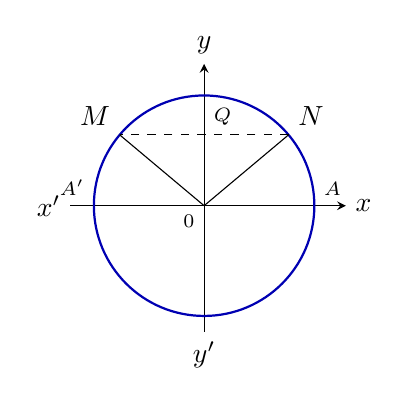
\begin{tikzpicture}[scale=1,>=stealth]
  \draw[->] (-1.7,0) -- (1.8,0) node[right] {$x$};
  \draw[->] (0,-1.6) -- (0,1.8) node[above] {$y$};
  \node[left] at (-1.7,0) {$x'$}; \node[below] at (0,-1.6) {$y'$};
  \draw[blue!70!black,thick] (0,0) circle (1.4);
  \draw (0,0) -- (40:1.4) node[above right] {$N$};
  \draw (0,0) -- (140:1.4) node[above left] {$M$};
  \draw[dashed] (40:1.4) -- (140:1.4);
  \node[above right] at (0,0.9) {\scriptsize $Q$};
  \node[above right] at (1.4,0) {\scriptsize $A$}; \node[above left] at (-1.4,0) {\scriptsize $A'$};
  \node[below left] at (0,0) {\scriptsize $0$};
\end{tikzpicture}
\end{center}
$\sin x$ ជាអរដោនេនៃចំណុច $M$ និង $\sin y$ ជាអរដោនេនៃចំណុច $N$ ។ ដោយ $\sin x = \sin y$ នោះ $M$ និង $N$ មានអរដោនេដូចគ្នា ។ ដូច្នេះ គេបានករណីពីរដូចខាងក្រោម ៖
\begin{itemize}
  \item បើ $M$ និង $N$ ត្រួតស៊ីគ្នា នោះ $x = y + 2k\pi$, $(k \in \mathbb{Z})$
  \item បើ $M$ និង $N$ ឆ្លុះគ្នាធៀបនឹងអ័ក្ស $(y'y)$ នោះមុំ $(\overrightarrow{OA}, \overrightarrow{ON})$ និងមុំ $(\overrightarrow{OA}, \overrightarrow{OM})$ ជាមុំបន្ថែមគ្នា ហើយ $\pi - y$ ជារង្វាស់នៃមុំ $(\overrightarrow{OA}, \overrightarrow{OM})$ ។ ដូច្នេះ $x = \pi - y + 2k\pi$, $(k \in \mathbb{Z})$ ។
\end{itemize}
\begin{formulaBox}[ជាទូទៅ]
គេបាន (II) $x$ និង $y$ ពីរចំនួនពិតមានស៊ីនុសដូចគ្នា $\sin x = \sin y$ លុះត្រាតែ $x = y + 2k\pi$ ឬ $x = \pi - y + 2k\pi$, $(k \in \mathbb{Z})$ ។
\end{formulaBox}

\section{សមីការត្រីកោណមាត្រ}

\subsection{ការដោះស្រាយសមីការ \texorpdfstring{$\cos x = a$}{cos x = a}}

\begin{example}[ឧទាហរណ៍ ១]
ដោះស្រាយសមីការ $\cos x = \dfrac{1}{2}$ ។

គេដឹងថា $\cos\dfrac{\pi}{3} = \dfrac{1}{2}$ សមីការអាចសរសេរ $\cos x = \cos\dfrac{\pi}{3}$ តែ $\cos\dfrac{\pi}{3} = \cos\left(-\dfrac{\pi}{3}\right)$ ។

ដូច្នេះ សមីការមានចម្លើយពីរគឺ $x = \dfrac{\pi}{3} + 2k\pi$, $x = -\dfrac{\pi}{3} + 2k\pi$, $(k \in \mathbb{Z})$ ។
\end{example}

\begin{example}[ឧទាហរណ៍ ២]
ដោះស្រាយសមីការ $\cos x = a$ ។ $a$ ជាចំនួនពិតដែលគេឱ្យ ៖
\begin{itemize}
  \item កាលណា $|a| > 1$ សមីការ $\cos x = a$ គ្មានចម្លើយ ព្រោះគ្រប់ចំនួន $x \in \mathbb{R}$, $-1 \le \cos x \le 1$ ។
  \item កាលណា $|a| \le 1$ គេបានករណីដូចខាងក្រោម ៖
\end{itemize}
ក្នុងរង្វង់ត្រីកោណមាត្រដែលមានផ្ចិត $O$ និង $A$ ជាចំណុចគល់នៃធ្នូ ហើយមុំ $(\overrightarrow{OA}, \overrightarrow{ON}) = \alpha$ ដែល $\cos\alpha = OP = a$ ។ ម្យ៉ាងវិញទៀត $a = OP = \cos(-\alpha)$ ដែល $-\alpha$ ជារង្វាស់នៃមុំ $(\overrightarrow{OA}, \overrightarrow{OM})$ ។ គេបាន
\begin{itemize}
  \item បើ $a \notin [-1, 1]$ សមីការ $\cos x = a$ គ្មានចម្លើយ ។
  \item បើ $a = 1$ ឬ $\cos x = 1$ នោះចុងធ្នូត្រួតស៊ីគ្នានឹងចំណុច $A$ ជាចម្លើយនៃសមីការ ។ ដូច្នេះ $x = 2k\pi$, $(k \in \mathbb{Z})$ ។
  \item បើ $a = -1$ ឬ $\cos x = -1$ នោះចុងធ្នូត្រួតស៊ីគ្នានឹងចំណុច $A'$ ជាចម្លើយនៃសមីការ ។ ដូច្នេះ $x = \pi + 2k\pi$, $(k \in \mathbb{Z})$ ។
  \item បើ $a \in\ ]-1, 1[$ មាន $\alpha$ តែមួយគត់ដែល $\cos\alpha = a = \cos x$ ។
\end{itemize}
ការដោះស្រាយសមីការ $\cos x = a$ គឺដោះស្រាយសមីការ $\cos x = \cos\alpha$ ។ តាមលក្ខណៈ (I) គេបាន ៖
\end{example}

\begin{formulaBox}[សមីការ $\cos x = \cos\alpha$]
ចម្លើយនៃសមីការ $\cos x = \cos\alpha$ មានពីរគឺ $x = \alpha + 2k\pi$ ឬ $x = -\alpha + 2k\pi$, $(k \in \mathbb{Z})$ ។
\end{formulaBox}

\begin{note}[សម្គាល់]
\begin{enumerate}[1]
  \item បើ $a = 0$ នោះ $\cos\alpha = 0$ ។ ចម្លើយរបស់សមីការ $\cos x = 0$ គឺ $x = \dfrac{\pi}{2} + k\pi$, $(k \in \mathbb{Z})$ ។
  \item តាមលក្ខណៈមុំពីរដែលមានកូស៊ីនុសដូចគ្នា លុះត្រាតែមុំទាំងពីរស្មើគ្នា ឬផ្ទុយគ្នានោះ គេអាចដោះស្រាយសមីការ $\cos u(x) = \cos v(x)$ សមមូល $u(x) = \pm v(x) + 2k\pi$, $(k \in \mathbb{Z})$ ដែល $u(x)$ និង $v(x)$ ជាអនុគមន៍នៃ $x$ ។
\end{enumerate}
\end{note}

\begin{example}[លំហាត់គំរូ ១]
ដោះស្រាយសមីការ $\cos\left(x - \dfrac{\pi}{4}\right) = \sin 3x$ រួចដៅចុងធ្នូនៃចម្លើយលើរង្វង់ត្រីកោណមាត្រ ។
\end{example}
\ans
តាមធ្នូបំពេញ គេបាន $\sin 3x = \cos\left(\dfrac{\pi}{2} - 3x\right)$ ដូច្នេះ $\cos\left(x - \dfrac{\pi}{4}\right) = \cos\left(\dfrac{\pi}{2} - 3x\right)$ នាំឱ្យ
\[
\begin{gathered}
x - \frac{\pi}{4} = \frac{\pi}{2} - 3x + 2k\pi \quad \text{ឬ}\\
x - \frac{\pi}{4} = -\left(\frac{\pi}{2} - 3x\right) + 2k\pi,\\
(k \in \mathbb{Z})
\end{gathered}
\]
គេបាន $4x = \dfrac{3\pi}{4} + 2k\pi$ ឬ $-2x = -\dfrac{\pi}{4} + 2k\pi$ ។ ដូច្នេះ $x = \dfrac{3\pi}{16} + \dfrac{k\pi}{2}$ ឬ $x = \dfrac{\pi}{8} - k\pi$, $(k \in \mathbb{Z})$ ។

គេអាចសរសេរ $\dfrac{\pi}{8} - k\pi$ ទៅជា $\dfrac{\pi}{8} + K\pi$ ដែល $K = -k$, ($k \in \mathbb{Z}$ ដូច្នេះ $K \in \mathbb{Z}$) ។

គេបាន (1) $x = \dfrac{3\pi}{16} + k\dfrac{\pi}{2}$
\begin{itemize}
  \item បើ $k = 0$, $x = \dfrac{3\pi}{16}$ ចុងធ្នូត្រង់ចំណុច $M_1$
  \item បើ $k = 1$, $x = \dfrac{3\pi}{16} + \dfrac{\pi}{2}$ ចុងធ្នូត្រង់ចំណុច $M'_1$
  \item បើ $k = 2$, $x = \dfrac{3\pi}{16} + \pi$ ចុងធ្នូត្រង់ចំណុច $M_2$
  \item បើ $k = 3$, $x = \dfrac{3\pi}{16} + \dfrac{3\pi}{2}$ ចុងធ្នូត្រង់ចំណុច $M'_2$
  \item បើ $k = 4$, $x = \dfrac{3\pi}{16} + 2\pi$ ចុងធ្នូត្រួតលើ $M_1$ ។
\end{itemize}
ដូច្នេះ (1) មានសំណុំចម្លើយចុងធ្នូបួនគឺ $M_1$, $M'_1$, $M_2$, $M'_2$ ។

ចំពោះ (2) $x = \dfrac{\pi}{8} + k\pi$
\begin{itemize}
  \item បើ $k = 0$, $x = \dfrac{\pi}{8}$ ចុងធ្នូត្រង់ចំណុច $N_1$
  \item បើ $k = 1$, $x = \dfrac{\pi}{8} + \pi$ ចុងធ្នូត្រង់ចំណុច $N'_1$
  \item បើ $k = 2$, $x = \dfrac{\pi}{8} + 2\pi$ ចុងធ្នូត្រង់ចំណុច $N_1$ ។
\end{itemize}
ដូច្នេះ (2) មានសំណុំចម្លើយចុងធ្នូពីរគឺ $N_1$ និង $N'_1$ ។
\begin{center}
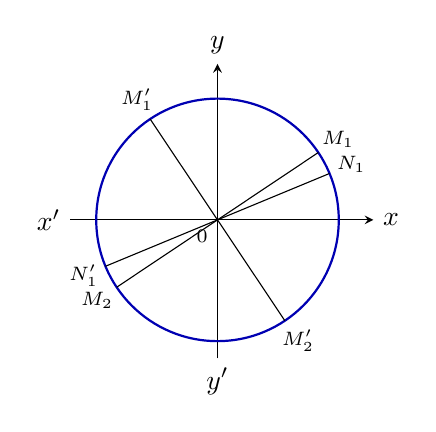
\begin{tikzpicture}[scale=1.1,>=stealth]
  \draw[->] (-1.7,0) -- (1.8,0) node[right] {$x$};
  \draw[->] (0,-1.6) -- (0,1.8) node[above] {$y$};
  \node[left] at (-1.7,0) {$x'$}; \node[below] at (0,-1.6) {$y'$};
  \draw[blue!70!black,thick] (0,0) circle (1.4);
  \foreach \a/\n in {33.75/{M_1},123.75/{M'_1},213.75/{M_2},303.75/{M'_2}} \draw (0,0) -- (\a:1.4) node[shift={(\a:0.3)}] {\scriptsize $\n$};
  \foreach \a/\n in {22.5/{N_1},202.5/{N'_1}} \draw (0,0) -- (\a:1.4) node[shift={(\a:0.3)}] {\scriptsize $\n$};
  \node[below left] at (0,0) {\scriptsize $0$};
\end{tikzpicture}
\end{center}

\begin{example}[លំហាត់គំរូ ២]
ដោះស្រាយសមីការ $1 + 3\cos x + \cos 2x = \cos 3x + 2\sin x \cdot \sin 2x$ ។
\end{example}
\ans
\[
\begin{aligned}
&1 + 3\cos x + \cos 2x = \cos 3x + 2\sin x \cdot \sin 2x\\
&3\cos x + 2\cos^2 x = \cos 3x + \cos x - \cos 3x\\
&\text{សមមូល} \quad 2\cos x + 2\cos^2 x = 0\\
&2\cos x(1 + \cos x) = 0\\
&\text{សមមូល} \quad \cos x = 0 \ \text{ឬ} \ \cos x = -1
\end{aligned}
\]
ដូច្នេះ សមីការមានឫស $x = \dfrac{\pi}{2} + k\pi$, $x = \pi + 2k\pi$ $(k \in \mathbb{Z})$ ។

\begin{pro}
ដោះស្រាយសមីការខាងក្រោម ៖
\begin{tasks}(2)
  \task $\cos\left(3x - \dfrac{\pi}{6}\right) = -1$
  \task $\cos\left(3x + \dfrac{\pi}{3}\right) = \cos\left(x - \dfrac{\pi}{6}\right)$
  \task $\cos\dfrac{\pi}{6}\cos x - \sin\dfrac{\pi}{6}\sin x = \dfrac{\sqrt{2}}{2}$
  \task $\sin\left(x - \dfrac{\pi}{4}\right) = \dfrac{1}{2}$ ។
\end{tasks}
\ans
\begin{enumerate}[a]
  \item $x = \dfrac{7\pi}{18} + \dfrac{2k\pi}{3}$, $(k \in \mathbb{Z})$
  \item $x = -\dfrac{\pi}{4} + k\pi$ ឬ $x = -\dfrac{\pi}{24} + \dfrac{k\pi}{2}$, $(k \in \mathbb{Z})$
  \item $x = \dfrac{\pi}{12} + 2k\pi$ ឬ $x = -\dfrac{5\pi}{12} + 2k\pi$, $(k \in \mathbb{Z})$
  \item $x = \dfrac{5\pi}{12} + 2k\pi$ ឬ $x = \dfrac{13\pi}{12} + 2k\pi$, $(k \in \mathbb{Z})$ ។
\end{enumerate}
\end{pro}

\subsection{ការដោះស្រាយសមីការ \texorpdfstring{$\sin x = a$}{sin x = a}}

\begin{example}[ឧទាហរណ៍ ១]
ដោះស្រាយសមីការ $\sin x = \dfrac{\sqrt{2}}{2}$ ។

គេដឹងថា $\sin\dfrac{\pi}{4} = \dfrac{\sqrt{2}}{2}$ សមីការអាចសរសេរ $\sin x = \sin\dfrac{\pi}{4}$ ។ ដូច្នេះ សមីការមានចម្លើយពីរគឺ
\[
\begin{gathered}
x = \frac{\pi}{4} + 2k\pi \ \text{ឬ} \ x = \pi - \frac{\pi}{4} + 2k\pi, \ (k \in \mathbb{Z})\\
\text{ឬ}\\
x = \frac{\pi}{4} + 2k\pi, \ x = \frac{3\pi}{4} + 2k\pi, \ (k \in \mathbb{Z}) \text{ ។}
\end{gathered}
\]
\end{example}

\begin{example}[ឧទាហរណ៍ ២]
ដោះស្រាយសមីការ $\sin x = a$ ។
\begin{itemize}
  \item កាលណា $|a| > 1$ សមីការ $\sin x = a$ គ្មានចម្លើយព្រោះគ្រប់ចំនួន $x \in \mathbb{R}$ ៖ $-1 \le \sin x \le 1$ ។
  \item កាលណា $|a| \le 1$ គេបានករណីដូចខាងក្រោម ៖
\end{itemize}
ក្នុងរង្វង់ត្រីកោណមាត្រដែលមានផ្ចិត $O$ និង $A$ ជាចំណុចគល់នៃធ្នូ ហើយ $(\overrightarrow{OA}, \overrightarrow{OM}) = \alpha$ ដែល $\sin\alpha = OQ = a$ ។ ម្យ៉ាងវិញទៀត $OQ = \sin(\pi - \alpha) = a$ ដែល $\pi - \alpha$ ជារង្វាស់នៃមុំ $(\overrightarrow{OA}, \overrightarrow{OM'})$ ។
\begin{center}
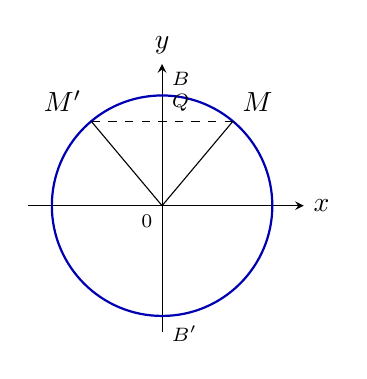
\begin{tikzpicture}[scale=1,>=stealth]
  \draw[->] (-1.7,0) -- (1.8,0) node[right] {$x$};
  \draw[->] (0,-1.6) -- (0,1.8) node[above] {$y$};
  \draw[blue!70!black,thick] (0,0) circle (1.4);
  \draw (0,0) -- (50:1.4) node[above right] {$M$};
  \draw (0,0) -- (130:1.4) node[above left] {$M'$};
  \draw[dashed] (50:1.4) -- (130:1.4);
  \node[above right] at (0,1.07) {\scriptsize $Q$};
  \node[above right] at (0,1.4) {\scriptsize $B$}; \node[below right] at (0,-1.4) {\scriptsize $B'$};
  \node[below left] at (0,0) {\scriptsize $0$};
\end{tikzpicture}
\end{center}
គេបាន
\begin{itemize}
  \item បើ $a \notin [-1, 1]$ សមីការ $\sin x = a$ គ្មានចម្លើយ ។
  \item បើ $a = 1$ ឬ $\sin x = 1$ នោះធ្នូទាំងឡាយណាដែលមានចុងត្រង់ចំណុច $B$ ជាចម្លើយនៃសមីការ ។ ដូច្នេះ $\sin x = 1$ សមមូល $x = \dfrac{\pi}{2} + 2k\pi$, $(k \in \mathbb{Z})$ ។
  \item បើ $a = -1$ ឬ $\sin x = -1$ នោះធ្នូទាំងឡាយដែលមានចុងត្រង់ចំណុច $B'$ ជាចម្លើយនៃសមីការ ។ ដូច្នេះ $\sin x = -1$ សមមូល $x = -\dfrac{\pi}{2} + 2k\pi$, $(k \in \mathbb{Z})$ ។
  \item បើ $a \in (-1, 1)$ មាន $\alpha$ តែមួយគត់ក្នុងចន្លោះ $\left(-\dfrac{\pi}{2}, \dfrac{\pi}{2}\right)$ ដែល $\sin\alpha = a = \sin x$ ។
\end{itemize}
ដោះស្រាយសមីការ $\sin x = a$ សមមូលនឹង $\sin x = \sin\alpha$ ។ តាមលក្ខណៈ (II) គេបាន ៖
\end{example}

\begin{formulaBox}[សមីការ $\sin x = \sin\alpha$]
សមីការ $\sin x = \sin\alpha$ មានចម្លើយពីរគឺ $x = \alpha + 2k\pi$ ឬ $x = \pi - \alpha + 2k\pi$, $(k \in \mathbb{Z})$ ។
\end{formulaBox}

\begin{note}[សម្គាល់]
\begin{enumerate}[1]
  \item បើ $a = 0$ នោះ $\sin x = 0$ ។ ចម្លើយរបស់សមីការគឺ $x = k\pi$, $(k \in \mathbb{Z})$ ។
  \item តាមលក្ខណៈមុំពីរដែលមានស៊ីនុសដូចគ្នា លុះត្រាតែមុំទាំងពីរស្មើគ្នា ឬបន្ថែមគ្នានោះ គេដោះស្រាយសមីការ $\sin u(x) = \sin v(x)$ សមមូល $u(x) = v(x) + 2k\pi$ ឬ $u(x) = \pi - v(x) + 2k\pi$ $(k \in \mathbb{Z})$ ដែល $u(x)$ និង $v(x)$ ជាអនុគមន៍នៃ $x$ ។
\end{enumerate}
\end{note}

\begin{example}[លំហាត់គំរូ ៣]
ដោះស្រាយ $\sin\dfrac{x}{2}\cos\dfrac{\pi}{3} - \cos\dfrac{x}{2}\sin\dfrac{\pi}{3} = \dfrac{1}{2}$ ។
\end{example}
\ans
គេបាន $\sin\dfrac{x}{2}\cos\dfrac{\pi}{3} - \cos\dfrac{x}{2}\sin\dfrac{\pi}{3} = \sin\left(\dfrac{x}{2} - \dfrac{\pi}{3}\right) = \dfrac{1}{2}$ ដោយ $\dfrac{1}{2} = \sin\dfrac{\pi}{6}$ គេបាន $\sin\left(\dfrac{x}{2} - \dfrac{\pi}{3}\right) = \sin\dfrac{\pi}{6}$ ។

សមីការមានចម្លើយពីរគឺ $\dfrac{x}{2} - \dfrac{\pi}{3} = \dfrac{\pi}{6} + 2k\pi$ ឬ $\dfrac{x}{2} - \dfrac{\pi}{3} = \pi - \dfrac{\pi}{6} + 2k\pi$ ។

ដូច្នេះ $x = \pi + 4k\pi$ ឬ $x = \dfrac{7\pi}{3} + 4k\pi$, $(k \in \mathbb{Z})$ ។

\begin{example}[លំហាត់គំរូ ៤]
ដោះស្រាយ $2\sin x\cos x + \sqrt{3} - 2\cos x - \sqrt{3}\sin x = 0$ ។
\end{example}
\ans
គេបាន $(2\sin x\cos x - \sqrt{3}\sin x) - (2\cos x - \sqrt{3}) = 0$
\[
\begin{gathered}
\sin x(2\cos x - \sqrt{3}) - (2\cos x - \sqrt{3}) = 0\\
\text{សមមូល}\\
(2\cos x - \sqrt{3})(\sin x - 1) = 0
\end{gathered}
\]
គេបាន $2\cos x - \sqrt{3} = 0$ ឬ $\sin x - 1 = 0$ នាំឱ្យ $\cos x = \dfrac{\sqrt{3}}{2}$ ឬ $\sin x = 1$ ។

ដូច្នេះ $\cos x = \cos\dfrac{\pi}{6}$ នាំឱ្យ $x = \pm\dfrac{\pi}{6} + 2k\pi$ ឬ $\sin x = 1$ នាំឱ្យ $x = \dfrac{\pi}{2} + 2k\pi$ ។

ដូច្នេះ សមីការមានចម្លើយ $x = \pm\dfrac{\pi}{6} + 2k\pi$ ឬ $x = \dfrac{\pi}{2} + 2k\pi$, $(k \in \mathbb{Z})$ ។

\begin{pro}
ដោះស្រាយសមីការខាងក្រោម ៖
\begin{tasks}(3)
  \task $\sin\left(2x + \dfrac{\pi}{4}\right) = 1$
  \task $\sin 2x = \sin\left(\dfrac{\pi}{3} - x\right)$
  \task $2\sin x\cos x - 3\sin 2x = 0$ ។
\end{tasks}
\ans
\begin{enumerate}[a]
  \item $x = \dfrac{\pi}{8} + k\pi$, $(k \in \mathbb{Z})$
  \item $x = \dfrac{\pi}{9} + \dfrac{2k\pi}{3}$ ឬ $x = \dfrac{2\pi}{3} + 2k\pi$, $(k \in \mathbb{Z})$
  \item $x = \dfrac{k\pi}{2}$, $(k \in \mathbb{Z})$ ។
\end{enumerate}
\end{pro}

\subsection{ការដោះស្រាយសមីការ \texorpdfstring{$\tan x = a$}{tan x = a}}

\begin{example}[ឧទាហរណ៍ ១]
ដោះស្រាយសមីការ $\tan x = -1$ ។

គេដឹងថា អនុគមន៍តង់សង់មានខួបស្មើនឹង $\pi$ ។ ដូច្នេះគេអាចរកចំនួនពិត $x$ មួយដែល $\tan x = -1$ ។ ដោយសមីការសរសេរ $\tan x = \tan\left(-\dfrac{\pi}{4}\right)$ ។ ដូច្នេះសមីការមានចម្លើយ $x = -\dfrac{\pi}{4} + k\pi$, $(k \in \mathbb{Z})$ បកស្រាយតាមក្រាបចម្លើយរបស់សមីការនេះជាអាប់ស៊ីសនៃចំណុចប្រសព្វរបស់ក្រាបនៃអនុគមន៍ $y = \tan x$ និងបន្ទាត់ដេក $y = -1$ ។
\end{example}

\begin{example}[ឧទាហរណ៍ ២]
ដោះស្រាយសមីការ $\tan x = t$ ។

គេមានរង្វង់ត្រីកោណមាត្រ $(C)$ ហើយ $(u'u)$ ជាអ័ក្សតង់សង់ដែលប៉ះរង្វង់ $(C)$ ត្រង់ $A$ ។ នៅលើ $(u'Au)$ គេដៅចំណុច $T$ ដោយ $AT = t$ ។ រកធ្នូ $\overset{\frown}{AM}$ ទាំងអស់ដែលមានតង់សង់ $t$ ។
\begin{center}
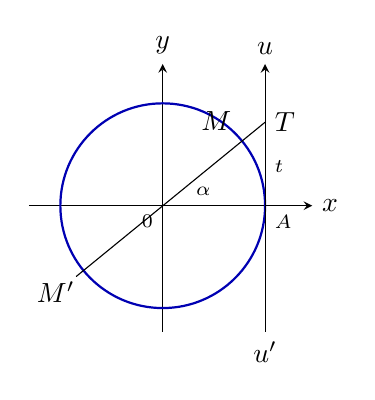
\begin{tikzpicture}[scale=1,>=stealth]
  \draw[->] (-1.7,0) -- (1.9,0) node[right] {$x$};
  \draw[->] (0,-1.6) -- (0,1.8) node[above] {$y$};
  \draw[blue!70!black,thick] (0,0) circle (1.3);
  \draw[->] (1.3,-1.6) -- (1.3,1.8) node[above] {$u$}; \node[below] at (1.3,-1.6) {$u'$};
  \draw (-1.1,-0.9) -- (1.3,1.06) node[right] {$T$};
  \node[above left] at (40:1.3) {$M$}; \node[below left] at (220:1.3) {$M'$};
  \node[below right] at (1.3,0) {\scriptsize $A$}; \node[below left] at (0,0) {\scriptsize $0$};
  \node at (20:0.55) {\scriptsize $\alpha$}; \node[right] at (1.3,0.5) {\scriptsize $t$};
\end{tikzpicture}
\end{center}
$\alpha$ ជារង្វាស់មួយនៃធ្នូ $\overset{\frown}{AM}$ ហើយចំណុច $M$ និង $M'$ ឆ្លុះគ្នាធៀបនឹង $O$ ។ ធ្នូចម្លើយត្រូវមានចុងត្រង់ $M$ និង $M'$ ។ ធ្នូទាំងអស់ដែលមានចុង $M$ មានរង្វាស់ $x = \alpha + 2k\pi$ ។ ធ្នូមួយដែលមានចុង $M'$ មានរង្វាស់ $\pi + \alpha$ ហើយធ្នូទាំងអស់ដែលមានចុង $M'$ មានរង្វាស់ $x = \pi + \alpha + 2k\pi$ ឬ $x = \alpha + (2k + 1)\pi$ ។ គេបានចម្លើយ $x = \alpha + k\pi$, $(k \in \mathbb{Z})$ ។
\end{example}

\begin{formulaBox}[ដូច្នេះ]
សមីការ $\tan x = a = \tan\alpha$ មានចម្លើយ $x = \alpha + k\pi$, $(k \in \mathbb{Z})$ ។
\end{formulaBox}

\begin{note}[សម្គាល់]
គេបាន $\tan u(x) = \tan v(x)$ សមមូល $u(x) = v(x) + k\pi$, $k \in \mathbb{Z}$ ដែល $u$ និង $v$ ជាអនុគមន៍នៃ $x$ ។
\end{note}

\begin{example}[ឧទាហរណ៍ ៣]
ដោះស្រាយសមីការ $\tan 3x = \tan\left(\dfrac{\pi}{3} - 2x\right)$ ។

គេបាន $\tan 3x = \tan\left(\dfrac{\pi}{3} - 2x\right)$ សមមូល $3x = \dfrac{\pi}{3} - 2x + k\pi$ សមមូល $5x = \dfrac{\pi}{3} + k\pi$, $(k \in \mathbb{Z})$ ។

សមីការមានចម្លើយ $x = \dfrac{\pi}{15} + k\dfrac{\pi}{5}$, $(k \in \mathbb{Z})$ ។
\end{example}

\begin{example}[លំហាត់គំរូ ៥]
ដោះស្រាយសមីការ $\tan x = -0.7456$ ។
\end{example}
\ans
តាមតារាងត្រីកោណមាត្រ គេបាន $\tan 36^\circ = 0.7265$ និង $\tan 37^\circ = 0.7536$ រកមុំ $\alpha'$ ដែល $\tan\alpha' = 0.7456$ ។

គេបាន $\tan 36^\circ < \tan\alpha' < \tan 37^\circ$ និង $\tan 37^\circ - \tan 36^\circ = 0.0271$, \ $\tan\alpha' - \tan 36^\circ = 0.0191$, \ $\alpha' > 36^\circ$ ។

គេត្រូវថែមលើ $36^\circ$ ចំនួន $\dfrac{60' \times 0.0191}{0.0271} \approx 42'$ ។ គេបាន $\alpha' = 36^\circ 42'$ ហើយ $-0.7456 = \tan(-36^\circ 42')$ ។

ដូច្នេះ $\tan x = \tan(-36^\circ 42')$ នាំឱ្យ $x = -36^\circ 42' + 180^\circ k$ $(k \in \mathbb{Z})$ ។

\begin{example}[លំហាត់គំរូ ៦]
ដោះស្រាយសមីការ $\dfrac{\tan\frac{\pi}{4} - \tan x}{1 + \tan x\tan\frac{\pi}{4}} = \sqrt{3}$ ។
\end{example}
\ans
ដោយ $\dfrac{\tan\frac{\pi}{4} - \tan x}{1 + \tan x\tan\frac{\pi}{4}} = \tan\left(\dfrac{\pi}{4} - x\right)$ និង $\tan\dfrac{\pi}{3} = \sqrt{3}$ សមីការអាចសរសេរ
\[
\begin{gathered}
\tan\left(x - \frac{\pi}{4}\right) = \tan\left(-\frac{\pi}{3}\right) \quad \text{នាំឱ្យ}\\
x - \frac{\pi}{4} = -\frac{\pi}{3} + k\pi
\end{gathered}
\]
ដូច្នេះ $x = -\dfrac{\pi}{12} + k\pi$, $(k \in \mathbb{Z})$ ជាចម្លើយរបស់សមីការ ។

\begin{pro}
ដោះស្រាយសមីការខាងក្រោម ៖
\begin{tasks}(2)
  \task $\tan x = \dfrac{1}{\sqrt{3}}$
  \task $\tan 3x = \sqrt{3}$
  \task $\dfrac{2\tan x}{1 - \tan^2 x} = \sqrt{3}$
  \task $\sqrt{3}\tan x = -1$ ។
\end{tasks}
\ans
\begin{tasks}(2)
  \task $x = \dfrac{\pi}{6} + k\pi$, $(k \in \mathbb{Z})$
  \task $x = \dfrac{\pi}{9} + \dfrac{k\pi}{3}$, $(k \in \mathbb{Z})$
  \task $x = \dfrac{\pi}{6} + \dfrac{k\pi}{2}$, $(k \in \mathbb{Z})$
  \task $x = -\dfrac{\pi}{6} + k\pi$, $(k \in \mathbb{Z})$ ។
\end{tasks}
\end{pro}

\subsection{ការដោះស្រាយសមីការ \texorpdfstring{$\cot x = m$}{cot x = m}}

សមីការ $\cot x = \cot\alpha$ អាចសរសេរ $\dfrac{1}{\tan x} = \dfrac{1}{\tan\alpha}$ នាំឱ្យ $\tan x = \tan\alpha$ ។ ដូច្នេះ គេអាចដោះស្រាយសមីការ $\cot x = m$ ដូចសមីការ $\tan x = t$ ខាងលើដែរ ។

ចំពោះសមីការ $\cot u(x) = \cot v(x)$ ដូចសមីការ $\tan u(x) = \tan v(x)$ ដែរ ។ សមីការ $\cot u(x) = \cot v(x)$ សមមូល $u(x) = v(x) + k\pi$, $(k \in \mathbb{Z})$ ដែល $u$ និង $v$ ជាអនុគមន៍នៃ $x$ ។

\begin{example}[ឧទាហរណ៍]
ដោះស្រាយសមីការ $\cot\left(2x + \dfrac{\pi}{3}\right) = \sqrt{3}$ ។

គេបាន $\cot\left(2x + \dfrac{\pi}{3}\right) = \sqrt{3} = \cot\dfrac{\pi}{6}$ នាំឱ្យ $2x + \dfrac{\pi}{3} = \dfrac{\pi}{6} + k\pi$, $(k \in \mathbb{Z})$ ។

ដូច្នេះ $2x = \dfrac{\pi}{6} - \dfrac{\pi}{3} + k\pi$ នាំឱ្យ $x = -\dfrac{\pi}{12} + \dfrac{k\pi}{2}$, $(k \in \mathbb{Z})$ ។
\end{example}

\begin{example}[លំហាត់គំរូ ៧]
ដោះស្រាយសមីការ $2(\cot 2x - \cot 3x) = \tan 2x + \cot 3x$ ។
\end{example}
\ans
លក្ខខណ្ឌនៃសមីការ $\sin 2x \ne 0$, $\sin 3x \ne 0$, $\cos 2x \ne 0$ ។ គេបាន
\[
\begin{gathered}
\cot 2x - \cot 3x = \frac{\sin(3x - 2x)}{\sin 2x\sin 3x} = \frac{\sin x}{\sin 2x\sin 3x},\\
\tan 2x + \cot 3x = \frac{\sin 3x\sin 2x + \cos 3x\cos 2x}{\cos 2x\sin 3x} = \frac{\cos x}{\cos 2x\sin 3x}
\end{gathered}
\]
សមីការក្លាយជា
\[
\begin{aligned}
&\frac{2\sin x}{\sin 2x\sin 3x} = \frac{\cos x}{\cos 2x\sin 3x} \quad \text{សមមូល} \quad 2\sin x\cos 2x\\
&= \sin 2x\cos x = 2\sin x\cos^2 x\\
&2\sin x(\cos 2x - \cos^2 x) = 0 \quad \text{សមមូល} \quad -2\sin^3 x = 0
\end{aligned}
\]
សមមូល $\sin x = 0$ ។ តាមលក្ខខណ្ឌនៃសមីការ $\sin 2x \ne 0$ នាំឱ្យ $\sin x \ne 0$ ។ ដូច្នេះសមីការគ្មានចម្លើយ ។

\begin{pro}
ដោះស្រាយសមីការខាងក្រោម ៖
\begin{tasks}(2)
  \task $\cot x = -\dfrac{1}{\sqrt{3}}$
  \task $\cot 3x = \sqrt{3}$
  \task $\cot\left(\dfrac{x}{2} - 3\right) = -1$
  \task $3\cot x - \sqrt{3} = 0$ ។
\end{tasks}
\ans
\begin{tasks}(2)
  \task $x = \dfrac{2\pi}{3} + k\pi$, $(k \in \mathbb{Z})$
  \task $x = \dfrac{\pi}{18} + \dfrac{k\pi}{3}$, $(k \in \mathbb{Z})$
  \task $x = 6 + \dfrac{3\pi}{2} + 2k\pi$, $(k \in \mathbb{Z})$
  \task $x = \dfrac{\pi}{3} + k\pi$, $(k \in \mathbb{Z})$ ។
\end{tasks}
\end{pro}

\section{វិសមីការត្រីកោណមាត្រ}

\begin{example}[ឧទាហរណ៍ ១]
ដោះស្រាយវិសមីការ $\sin x - \dfrac{1}{2} \ge 0$ ។

វិសមីការអាចសរសេរ $\sin x \ge \dfrac{1}{2}$ តែ $\sin\dfrac{\pi}{6} = \dfrac{1}{2} = \sin\dfrac{5\pi}{6}$ ។ នៅលើរង្វង់ត្រីកោណមាត្រ គេមានចំណុច $M$ និង $M'$ ដែលធ្នូ $\overset{\frown}{AM} = \dfrac{\pi}{6}$ និងធ្នូ $\overset{\frown}{AM'} = \dfrac{5\pi}{6}$ ។ គេសង្កេតឃើញស៊ីនុសនៃមួយចំនួនធំជាង ឬស្មើ $\dfrac{1}{2}$ លុះត្រាតែរូបភាពនៃចំនួននោះលើធ្នូ $\overset{\frown}{MBM'}$ រួមទាំងចំណុច $M$ និង $M'$ ។
\begin{center}
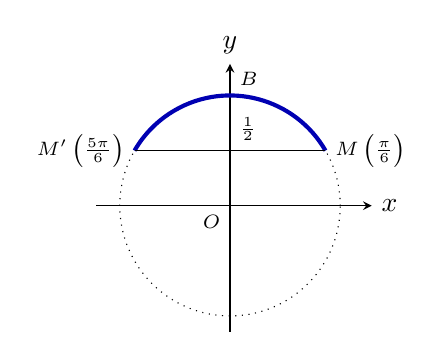
\begin{tikzpicture}[scale=1,>=stealth]
  \draw[->] (-1.7,0) -- (1.8,0) node[right] {$x$};
  \draw[->] (0,-1.6) -- (0,1.8) node[above] {$y$};
  \draw[dotted] (0,0) circle (1.4);
  \draw[blue!70!black,line width=1.5pt] (30:1.4) arc (30:150:1.4);
  \draw (30:1.4) node[right] {\scriptsize $M\left(\frac{\pi}{6}\right)$} -- (150:1.4) node[left] {\scriptsize $M'\left(\frac{5\pi}{6}\right)$};
  \node[above right] at (0,0.7) {\scriptsize $\frac{1}{2}$};
  \node[above right] at (0,1.4) {\scriptsize $B$}; \node[below left] at (0,0) {\scriptsize $O$};
\end{tikzpicture}
\end{center}
ដូច្នេះចម្លើយនៃវិសមីការ $\sin x - \dfrac{1}{2} \ge 0$ គឺ $\dfrac{\pi}{6} + 2k\pi \le x \le \dfrac{5\pi}{6} + 2k\pi$, $(k \in \mathbb{Z})$ ។
\end{example}

\begin{formulaBox}[ជាទូទៅ]
\begin{itemize}
  \item វិសមីការ $\sin x \le a$ គ្មានចម្លើយ កាលណា $a < -1$ ហើយបើ $-1 \le a \le 1$ មានចម្លើយ $-\pi - \alpha + 2k\pi \le x \le \alpha + 2k\pi$ ។
  \item វិសមីការ $\sin x \ge a$ គ្មានចម្លើយ កាលណា $a > 1$ ហើយបើ $-1 \le a \le 1$ មានចម្លើយ $\alpha + 2k\pi \le x \le \pi - \alpha + 2k\pi$ ។
\end{itemize}
(ដែល $\alpha \in \left[-\frac{\pi}{2}, \frac{\pi}{2}\right]$, $\sin\alpha = a$)
\end{formulaBox}

\begin{example}[ឧទាហរណ៍ ២]
ដោះស្រាយវិសមីការ $2\cos x + 1 < 0$ ។ វិសមីការអាចសរសេរ $\cos x < -\dfrac{1}{2}$ តែ $\cos\dfrac{2\pi}{3} = -\dfrac{1}{2} = \cos\dfrac{4\pi}{3}$ ។

នៅលើរង្វង់ត្រីកោណមាត្រ គេមានចំណុច $M$ និង $M'$ ដែលធ្នូ $\overset{\frown}{AM} = \dfrac{2\pi}{3}$ និងធ្នូ $\overset{\frown}{AM'} = \dfrac{4\pi}{3}$ ។ គេសង្កេតឃើញថា កូស៊ីនុសនៃមួយចំនួនតូចជាង $-\dfrac{1}{2}$ លុះត្រាតែរូបភាពនៃចំនួននោះលើធ្នូ $\overset{\frown}{MA'M'}$ លើកលែងចំណុច $M$ និង $M'$ ។
\begin{center}
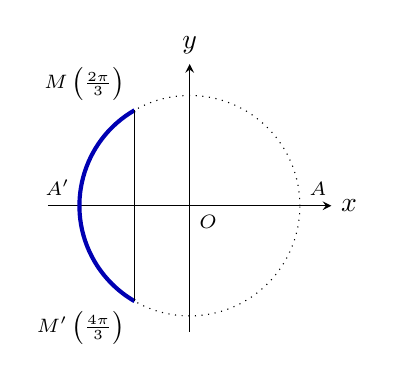
\begin{tikzpicture}[scale=1,>=stealth]
  \draw[->] (-1.8,0) -- (1.8,0) node[right] {$x$};
  \draw[->] (0,-1.6) -- (0,1.8) node[above] {$y$};
  \draw[dotted] (0,0) circle (1.4);
  \draw[blue!70!black,line width=1.5pt] (120:1.4) arc (120:240:1.4);
  \draw (120:1.4) node[above left] {\scriptsize $M\left(\frac{2\pi}{3}\right)$} -- (240:1.4) node[below left] {\scriptsize $M'\left(\frac{4\pi}{3}\right)$};
  \node[above left] at (-1.4,0) {\scriptsize $A'$}; \node[above right] at (1.4,0) {\scriptsize $A$};
  \node[below right] at (0,0) {\scriptsize $O$};
\end{tikzpicture}
\end{center}
ដូច្នេះចម្លើយនៃវិសមីការ $2\cos x + 1 < 0$ គឺ $\dfrac{2\pi}{3} + 2k\pi < x < \dfrac{4\pi}{3} + 2k\pi$, $(k \in \mathbb{Z})$ ។
\end{example}

\begin{formulaBox}[ជាទូទៅ]
\begin{itemize}
  \item វិសមីការ $\cos x \le a$ គ្មានចម្លើយ កាលណា $a < -1$ ហើយបើ $-1 \le a \le 1$ មានចម្លើយ $\alpha + 2k\pi \le x \le 2\pi - \alpha + 2k\pi$, $(k \in \mathbb{Z})$ ។
  \item វិសមីការ $\cos x \ge a$ គ្មានចម្លើយកាលណា $a > 1$ ហើយបើ $-1 \le a \le 1$ មានចម្លើយ $-\alpha + 2k\pi \le x \le \alpha + 2k\pi$, $(k \in \mathbb{Z})$ ។
\end{itemize}
(ដែល $\alpha \in [0, \pi]$, $\cos\alpha = a$)
\end{formulaBox}

\begin{note}[ករណីពិសេស]
វិសមីការ $\sin x > 0$ មានចម្លើយ $2k\pi < x < \pi + 2k\pi$, $(k \in \mathbb{Z})$ ។
\end{note}

\begin{example}[ឧទាហរណ៍ ៣]
ដោះស្រាយវិសមីការ $\tan x \ge -1$ ។ ដោយ $\tan\left(-\dfrac{\pi}{4}\right) = -1 = \tan\dfrac{3\pi}{4}$ ។

នៅលើរង្វង់ត្រីកោណមាត្រគេមានចំណុច $M$ និង $M'$ ដែល $\overset{\frown}{AM} = -\dfrac{\pi}{4}$, $\overset{\frown}{AM'} = \dfrac{3\pi}{4}$ ។ គេសង្កេតឃើញថាតង់សង់នៃមួយចំនួនធំជាង ឬស្មើ $-1$ លុះត្រាតែរូបភាពនៃចំនួននោះនៅលើធ្នូ $\overset{\frown}{MAB}$ ឬ $\overset{\frown}{M'A'B'}$ ។

ដូច្នេះ វិសមីការ $\tan x \ge -1$ មានចម្លើយ $-\dfrac{\pi}{4} + k\pi \le x < \dfrac{\pi}{2} + k\pi$, $(k \in \mathbb{Z})$ ។
\end{example}

\begin{formulaBox}[ជាទូទៅ]
គេបាន $\tan x \le a$ មានចម្លើយ $-\dfrac{\pi}{2} + k\pi < x \le \alpha + k\pi$ ។

$\tan x \ge a$ មានចម្លើយ $\alpha + k\pi \le x < \dfrac{\pi}{2} + k\pi$, $(k \in \mathbb{Z})$ ។
\end{formulaBox}

\begin{note}[សម្គាល់]
ដំណោះស្រាយវិសមីការ $\cot x$ ដូចគ្នានឹងដំណោះស្រាយវិសមីការ $\tan x$ ដែរ ។
\end{note}

\begin{formulaBox}[ជាទូទៅ]
ដើម្បីដោះស្រាយវិសមីការដែលមានរាង $\sin x \ge a$, $\cos x < a$, $\tan x > a$, $\cot x < a \ldots$ គេត្រូវ
\begin{itemize}
  \item រក $\alpha$ ដែល $\sin\alpha = a$, $\cos\alpha = a$, $\tan\alpha = a$, $\cot\alpha = a$
  \item ដៅចុងធ្នូតាមតម្លៃ $\alpha$ រួចបកស្រាយដោយប្រើរង្វង់ត្រីកោណមាត្រ
  \item ទាញរកសំណុំចម្លើយ ។
\end{itemize}
\end{formulaBox}

របៀបបំប្លែងអង្គទី $1$ នៃវិសមីការ គឺមានរបៀបដូចសមីការត្រីកោណមាត្រដែរ គេយករូបមន្តត្រីកោណមាត្រមកប្រើ ។

\begin{example}[លំហាត់គំរូ ៨]
ដោះស្រាយវិសមីការ $\sin\left(x - \dfrac{\pi}{3}\right) > \sin x$ ។
\end{example}
\ans
វិសមីការអាចសរសេរ
\[
\begin{aligned}
&\sin x - \sin\left(x - \frac{\pi}{3}\right) < 0\\
&2\sin\frac{x - x + \frac{\pi}{3}}{2}\cos\frac{x + x - \frac{\pi}{3}}{2} < 0\\
&2\sin\frac{\pi}{6}\cos\left(x - \frac{\pi}{6}\right) < 0 \quad \Leftrightarrow \quad \cos\left(x - \frac{\pi}{6}\right) < 0\\
&\frac{\pi}{2} + 2k\pi < x - \frac{\pi}{6} < \pi + \frac{\pi}{2} + 2k\pi, \qquad \frac{2\pi}{3}\\
&\quad + 2k\pi < x < \frac{5\pi}{3} + 2k\pi, \ (k \in \mathbb{Z}) \text{ ។}
\end{aligned}
\]

\begin{example}[លំហាត់គំរូ ៩]
ដោះស្រាយវិសមីការ $2\sin^2 x + 3\sin x - 2 \ge 0$ ។
\end{example}
\ans
តាង $t = \sin x$ ។ វិសមីការអាចសរសេរ $2t^2 + 3t - 2 \ge 0$ ឬ $(2t - 1)(t + 2) \ge 0$ ។

គេទាញ $t \le -2$ ឬ $t \ge \dfrac{1}{2}$ ដោយ $-1 \le t \le 1$ យើងយកតែ $\dfrac{1}{2} \le t \le 1$, \ $t = \sin x \ge \dfrac{1}{2}$ ។

ដោយ $\sin\dfrac{\pi}{6} = \dfrac{1}{2} = \sin\dfrac{5\pi}{6}$ គេបាន $\dfrac{\pi}{6} + 2k\pi \le x \le \dfrac{5\pi}{6} + 2k\pi$, $(k \in \mathbb{Z})$ ជាសំណុំចម្លើយនៃវិសមីការ ។

\begin{pro}
ដោះស្រាយវិសមីការខាងក្រោម ៖
\begin{tasks}(2)
  \task $2\cos x \ge -\sqrt{2}$
  \task $\cos 2x > \cos\dfrac{2\pi}{3}$
  \task $\sqrt{2}\cos x - 1 < 0$
  \task $\sin\left(\dfrac{\pi}{2} - x\right) < \cos\left(\dfrac{\pi}{2} + \dfrac{x}{2}\right)$
  \task $\cot x < \dfrac{\sqrt{3}}{3}$ ។
\end{tasks}
\ans
\begin{enumerate}[a]
  \item $-\dfrac{3\pi}{4} + 2k\pi \le x \le \dfrac{3\pi}{4} + 2k\pi$
  \item $-\dfrac{\pi}{3} + k\pi < x < \dfrac{\pi}{3} + k\pi$
  \item $\dfrac{\pi}{4} + 2k\pi < x < \dfrac{7\pi}{4} + 2k\pi$
  \item[ង.] $\dfrac{\pi}{3} + k\pi < x < \pi + k\pi$, \ $(k \in \mathbb{Z})$ ។
\end{enumerate}
\end{pro}

\section*{មេរៀនសង្ខេប ជំពូកទី ៣}
\begin{note}[មេរៀនសង្ខេប]
\begin{enumerate}[1]
  \item \textbf{រូបមន្តផលបូកនិងផលដក} \
  $\cos(\alpha \pm \beta) = \cos\alpha\cos\beta \mp \sin\alpha\sin\beta$, \ $\sin(\alpha \pm \beta) = \sin\alpha\cos\beta \pm \sin\beta\cos\alpha$, \ $\tan(\alpha \pm \beta) = \dfrac{\tan\alpha \pm \tan\beta}{1 \mp \tan\alpha\tan\beta}$ ។
  \item \textbf{រូបមន្តមុំឌុប} \ $\sin 2\alpha = 2\sin\alpha\cos\alpha$, \ $\cos 2\alpha = \cos^2\alpha - \sin^2\alpha = 1 - 2\sin^2\alpha = 2\cos^2\alpha - 1$ ។
  \item \textbf{រូបមន្តកន្លះមុំ} \ $\sin\alpha = 2\sin\dfrac{\alpha}{2}\cos\dfrac{\alpha}{2}$, \ $\cos^2\dfrac{\alpha}{2} = \dfrac{1 + \cos\alpha}{2}$, \ $\sin^2\dfrac{\alpha}{2} = \dfrac{1 - \cos\alpha}{2}$, \ $\tan\dfrac{\alpha}{2} = \dfrac{\sin\alpha}{1 + \cos\alpha}$ ។ បើ $\tan\dfrac{\alpha}{2} = t$ គេបាន $\cos\alpha = \dfrac{1 - t^2}{1 + t^2}$, $\sin\alpha = \dfrac{2t}{1 + t^2}$, $\tan\alpha = \dfrac{2t}{1 - t^2}$ ។
  \item \textbf{រូបមន្តបំប្លែង} \ $\sin\alpha\sin\beta = \dfrac{1}{2}[\cos(\alpha - \beta) - \cos(\alpha + \beta)]$, \ $\cos\alpha\cos\beta = \dfrac{1}{2}[\cos(\alpha + \beta) + \cos(\alpha - \beta)]$, \ $\sin\alpha\cos\beta = \dfrac{1}{2}[\sin(\alpha + \beta) + \sin(\alpha - \beta)]$ ។
  \item \textbf{បំប្លែងពីផលបូកទៅផលគុណ} \ $\cos p + \cos q = 2\cos\dfrac{p + q}{2}\cos\dfrac{p - q}{2}$, \ $\cos p - \cos q = -2\sin\dfrac{p + q}{2}\sin\dfrac{p - q}{2}$, \ $\sin p + \sin q = 2\sin\dfrac{p + q}{2}\cos\dfrac{p - q}{2}$, \ $\sin p - \sin q = 2\sin\dfrac{p - q}{2}\cos\dfrac{p + q}{2}$, \ $\tan p \pm \tan q = \dfrac{\sin(p \pm q)}{\cos p\cos q}$ ។
  \item សមីការ $\cos x = \cos\alpha$ មានចម្លើយពីរគឺ $x = \alpha + 2k\pi$ និង $x = -\alpha + 2k\pi$ $(k \in \mathbb{Z})$ ។
  \item សមីការ $\sin x = \sin\alpha$ មានចម្លើយពីរគឺ $x = \alpha + 2k\pi$ និង $x = \pi - \alpha + 2k\pi$, $(k \in \mathbb{Z})$ ។
  \item សមីការ $\tan x = \tan\alpha$ មានចម្លើយ $x = \alpha + k\pi$ ។
  \item សមីការ $\cot x = \cot\alpha$ មានចម្លើយ $x = \alpha + k\pi$, $(k \in \mathbb{Z})$ ។
  \item វិសមីការ ៖ $\sin x \le a$ ៖ $-\pi - \alpha + 2k\pi \le x \le \alpha + 2k\pi$; \ $\sin x \ge a$ ៖ $\alpha + 2k\pi \le x \le \pi - \alpha + 2k\pi$; \ $\cos x \le a$ ៖ $\alpha + 2k\pi \le x \le 2\pi - \alpha + 2k\pi$; \ $\cos x \ge a$ ៖ $-\alpha + 2k\pi \le x \le \alpha + 2k\pi$; \ $\tan x \le a$ ៖ $-\dfrac{\pi}{2} + k\pi < x \le \alpha + k\pi$; \ $\tan x \ge a$ ៖ $\alpha + k\pi \le x < \dfrac{\pi}{2} + k\pi$ ។
\end{enumerate}
\end{note}

\section*{លំហាត់ជំពូកទី ៣}
\begin{enumerate}[1]
  \item អង្កត់ធ្នូ $AB$ ចែករង្វង់មួយដែលមានកាំស្មើនឹង $2$ cm ជាពីរអង្កត់ ។ គេដឹងថា $AB$ ស្កាត់ធ្នូដែលមានមុំផ្ចិត $= 60^\circ$ ។ គណនា
  \begin{enumerate}[a]
    \item ក្រឡាផ្ទៃចម្រៀកថាស $AOB$ ។
    \item ក្រឡាផ្ទៃត្រីកោណ $AOB$ ។
    \item ក្រឡាផ្ទៃអង្កត់ថាសតូច (ផ្នែកតូច) ។
  \end{enumerate}
  \item គណនា
  \begin{tasks}(3)
    \task $\sin 960^\circ$
    \task $\cos 1215^\circ$
    \task $\sin 2940^\circ$
    \task $\cos\dfrac{13\pi}{6}$
    \task $\tan\left(-\dfrac{19}{4}\pi\right)$
    \task $\sin\left(-\dfrac{17}{3}\pi\right)$ ។
  \end{tasks}
  \item គណនា
  \begin{enumerate}[a]
    \item $\sin\theta + \sin\left(\theta + \dfrac{\pi}{2}\right) + \sin(\theta + \pi) + \sin\left(\theta + \dfrac{3}{2}\pi\right)$
    \item $\cos\dfrac{20}{3}\pi\tan\dfrac{7}{4}\pi + \sin\dfrac{5}{2}\pi\cos(-3\pi)$
    \item $\sin\left(\dfrac{\pi}{2} - \theta\right) + \cos\left(\dfrac{\pi}{2} + 2\theta\right) + \sin(\pi - 2\theta) + \cos(\pi - \theta)$ ។
  \end{enumerate}
  \item គេមាន $\tan\alpha + \tan\beta + \tan\gamma = \tan\alpha\tan\beta\tan\gamma$ $\left(-\dfrac{\pi}{2} < \alpha, \beta, \gamma < \dfrac{\pi}{2}\right)$ ។ គណនាមុំ $(\alpha + \beta + \gamma)$ ។
  \item គេមាន $\alpha = \cos 10^\circ$, $\beta = \cos 50^\circ$, $\gamma = \cos 70^\circ$ ។ គណនា $\alpha - \beta - \gamma$, $\alpha^2 - \beta\gamma$ និង $\alpha^2 + \beta^2 + \gamma^2$ ។
  \item បង្ហាញថា
  \begin{tasks}(2)
    \task $(1 - \sin A + \cos A)^2 = 2(1 - \sin A)(1 + \cos A)$
    \task $\cot A + \tan A = \dfrac{1}{\sin A\cos A}$
    \task $(\tan\theta + \sin\theta)(\tan\theta - \sin\theta) = \tan^2\theta\sin^2\theta$
    \task $\left(1 + \dfrac{1}{\sin\theta}\right)(1 - \sin\theta) = \cos\theta\cot\theta$ ។
  \end{tasks}
  \item ដោះស្រាយសមីការខាងក្រោម ៖
  \begin{tasks}(2)
    \task $4\cos^2 x - \cos 2x - 4\cos x + 1 = 0$
    \task $\sin^2 2x - \cos^2 8x = 0.5\cos 10x$
    \task $1 + \sin x + \cos x + \sin 2x + \cos 2x = 0$
    \task $\sin^4 x + \cos^4 x - \cos 2x + \dfrac{1}{4}\sin^2 2x - 2 = 0$
    \task $\sin^{2007} x + \cos^{2007} x = 1$
    \task $\tan x = \cot x + 2\cot^2 2x$ ។
  \end{tasks}
  \item
  \begin{enumerate}[a]
    \item គេឱ្យ $2\sin A\cos A + (\cos A + \sin A)^2 - (2\cos A + \sin A)^2 = p\sin^2 A + q$ ។ រកតម្លៃនៃចំនួនថេរ $p$ និង $q$ ។
    \item គេឱ្យ $\sin x\cos x(5\tan x + 2\cot x) = a + b\sin^2 x$ ។ រកតម្លៃនៃចំនួនថេរ $a$ និង $b$ ។
  \end{enumerate}
  \item ដោះស្រាយវិសមីការខាងក្រោម ដោយដឹងថា $0 \le x < 2\pi$
  \begin{tasks}(2)
    \task $\cos\left(x + \dfrac{\pi}{3}\right) \ge -\dfrac{1}{2}$
    \task $\tan\left(x - \dfrac{\pi}{6}\right) \ge -1$ ។
  \end{tasks}
  \item ដោះស្រាយសមីការនិងវិសមីការខាងក្រោម ៖
  \begin{tasks}(2)
    \task $2\sin^2\theta - \sqrt{2}\cos\theta = 0$
    \task $2\cos^2\theta + \sqrt{3}\sin\theta + 1 > 0$ ។
  \end{tasks}
  \item គេឱ្យ $\triangle ABC$ មានមុំ $3$ ជាមុំស្រួច ។
  \begin{enumerate}[a]
    \item បង្ហាញថា $\tan A + \tan B + \tan C = \tan A \cdot \tan B \cdot \tan C$
    \item តាង $T = \tan A + \tan B + \tan C$ ។ បង្ហាញថា $T \ge 3\sqrt{3}$ ។
  \end{enumerate}
\end{enumerate}

\section*{លំហាត់អនុវត្តន៍}
\begin{enumerate}[1]
  \item ដោះស្រាយសមីការខាងក្រោម ៖
  \begin{tasks}(2)
    \task $\sin\theta = \dfrac{\sqrt{3}}{2}$
    \task $\cos\theta = -\dfrac{1}{\sqrt{2}}$
    \task $\cos\left(4x + \dfrac{\pi}{3}\right) = \cos\left(x - \dfrac{\pi}{6}\right)$
    \task $\cos^2 x = 1$
    \task $\sin\sqrt{x} = -1$
    \task $\cot x = 1$
    \task $\dfrac{1}{\cos 2x} = \sqrt{2}$
    \task $2\sin\left(2x - \dfrac{\pi}{3}\right) = 1$
    \task $\cos\left(2x - \dfrac{\pi}{3}\right) = \dfrac{\sqrt{3}}{2}$
    \task $\tan^3\left(x - \dfrac{\pi}{4}\right) = \tan(x - 1)$
    \task $\cot\left(2x + \dfrac{\pi}{3}\right) = 2$
    \task $\dfrac{2\tan x}{1 - \tan^2 x} = 5$ ។
  \end{tasks}
  \item ដោះស្រាយសមីការខាងក្រោម ៖
  \begin{tasks}(2)
    \task $\tan^3 3x - 2\sin^3 3x = 0$
    \task $\cos\left(\dfrac{3\pi}{2} + x\right) = \sqrt{2}\sin x\cos x$
    \task $\sin 2x = (\cos x - \sin x)^2$
    \task $\sqrt{3}\sin(x + \sin x) = \dfrac{1}{\cos x}$
    \task $\sin 2x + \tan x = 2$
    \task $\dfrac{\sqrt{3}}{\cos^2 x} = 4\tan x$
    \task $\dfrac{1 + \sin x}{1 + \cos x} = \dfrac{1}{2}$
    \task $\sin 3x + \cos 2x = 1 + 2\sin x\cos 2x$
    \task $\sin 2(x - \pi) - \sin(3x - \pi) = \sin x$
    \task $\tan x + \cot x = 2(\sin 2x + \cos 2x)$
    \task $\dfrac{\sin x + \sin 2x + \sin 3x}{\cos x + \cos 2x + \cos 3x} = \sqrt{3}$ ។
  \end{tasks}
  \item ដោះស្រាយវិសមីការខាងក្រោម ៖
  \begin{tasks}(2)
    \task $2\cos\theta \le -\sqrt{2}$
    \task $-\sqrt{2}\sin\theta + 1 \ge 0$
    \task $\sqrt{3}\tan\theta - 1 < 0$
    \task $\sin\left(2\theta + \dfrac{\pi}{3}\right) = -\dfrac{\sqrt{3}}{2}$ \ $(-\pi \le \theta < \pi)$
    \task $\cos\left(\dfrac{1}{2}\theta - \dfrac{\pi}{3}\right) \le \dfrac{1}{\sqrt{2}}$ \ $(0 \le \theta < 2\pi)$ ។
  \end{tasks}
  \item រកគ្រប់មុំចន្លោះ $0^\circ$ និង $360^\circ$ ដែលផ្ទៀងផ្ទាត់សមីការ
  \begin{tasks}(2)
    \task $2\tan y = 5\sin y$
    \task $8\sin x\cos x = \sin x$
    \task $4\sin^2 x = 6 - 9\cos x$
    \task $3\cos y + \cot y = 0$
    \task $2\sin 2x + 1 = 0$
    \task $6\sin x - 8\sin^2 x = 5\cos^2 x$
    \task $2\cot 2x = 5$
    \task $3\sin y\tan y + 8 = 0$
    \task $3\cos^2 y = 7\sin y + 5$
    \task $\cot\left(\dfrac{z}{2}\right) - 2\cos\left(\dfrac{z}{2}\right) = 0$
    \task $\tan(x - 30^\circ)\tan 50^\circ = 0$ ។
  \end{tasks}
  \item គេឱ្យ $x = 3\sin\theta - 2\cos\theta$ និង $y = 3\cos\theta + 2\sin\theta$
  \begin{enumerate}[a]
    \item រកតម្លៃនៃមុំស្រួច $\theta$ ចំពោះ $x = y$
    \item បង្ហាញថា $x^2 + y^2$ ជាចំនួនថេរចំពោះគ្រប់តម្លៃនៃ $\theta$ ។
  \end{enumerate}
  \item គេឱ្យត្រីកោណ $ABC$ មាន $\dfrac{\sin A + \cos B}{\sin B + \cos A} = \tan A$ ។ បង្ហាញថា $\triangle ABC$ ជាត្រីកោណកែង ។
  \item គេឱ្យត្រីកោណ $ABC$ មាន $\dfrac{\sin C}{\sin B} = 2\cos A$ ។ រកប្រភេទនៃ $\triangle ABC$ ។
  \item គេឱ្យ $\triangle ABC$ មានមុំបំពេញលក្ខខណ្ឌ $\tan B + \tan C = 2\cot\dfrac{A}{2}$ ។ បង្ហាញថា $\triangle ABC$ ជាត្រីកោណសមបាត ។
\end{enumerate}
